\documentclass{beamer}
%
% Choose how your presentation looks.
%
% For more themes, color themes and font themes, see:
% http://deic.uab.es/~iblanes/beamer_gallery/index_by_theme.html
%
\mode<presentation>
{
  \usetheme{Darmstadt}      % or try Darmstadt, Madrid, Warsaw, ...
  \usecolortheme{beaver} % or try albatross, beaver, crane, ...
  \usefonttheme{serif}  % or try serif, structurebold, ...
  \setbeamertemplate{navigation symbols}{}
  \setbeamertemplate{caption}[numbered]
} 

\usepackage[english]{babel}
\usepackage[utf8x]{inputenc}
\usepackage{xcolor}
\usepackage{listings}
\usepackage{algorithm}
\usepackage{algpseudocode}
\usepackage[citestyle=numeric]{biblatex}

\addbibresource{thesis_references.bib}

\lstset
{
    language=[LaTeX]TeX,
    breaklines=true,
    basicstyle=\tt\scriptsize,
    %commentstyle=\color{green}
    keywordstyle=\color{blue},
    %stringstyle=\color{black}
    identifierstyle=\color{magenta},
}

\title[Management Interface]{API design and implementation of a management interface for SDN whitebox switches }
\author{Rubens Jesus Alves Figueiredo}
\institute{FEUP}
\date{\today}

\AtBeginSection[]
{
  \begin{frame}<beamer>
    \frametitle{Outline}
    \tableofcontents[currentsection,currentsubsection]
  \end{frame}
}

\graphicspath{{../doc/figures/}}

\begin{document}

\begin{frame}
  \titlepage
        \includegraphics[width=.3\textwidth,left]{{uporto-feup}}
        \includegraphics[width=.2\textwidth,height=2cm,right]{{bisdn-logo}}
\end{frame}

% Uncomment these lines for an automatically generated outline.
\begin{frame}{Outline}
  \tableofcontents
\end{frame}

\section{Introduction}

\begin{frame}{Motivation}
    \begin{figure}
        \centering
        \includegraphics[width=.8\textwidth]{presentation/google_data_center}
    \end{figure}
\end{frame}

\begin{frame}{Motivation}
	\begin{itemize}
  		\item Large scale Data Center Networks are hard to operate at a highly efficient and cost effective way
        \item Individually managing each network device (switches, server, ...) is a time consuming task
  		\item Move to cloud based environments requires planning and research to create a scalable and simple environment
	\end{itemize}
\end{frame}

\begin{frame}{Software Defined Networking}
    \begin{itemize}
    \item Networking services are bound to a fast changing environment, there is a need for a network design methodology that supports this
        fast evolution
        \pause
    \item \textbf{Software Defined Networking} is a solution that provides:
        \pause
    \item \textbf{Separation of control and data planes} 
        \pause
    \item \textbf{Centralization of network management functions}
    \end{itemize}
\end{frame}

\begin{frame}
    \begin{figure}[!tbph]
      \centering
      \subfloat{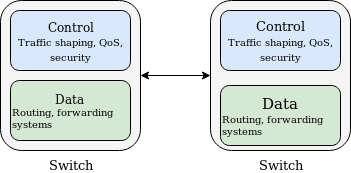
\includegraphics[width=0.4\textwidth]{bib/network_trad}\label{fig:net_trad}}
      \subfloat{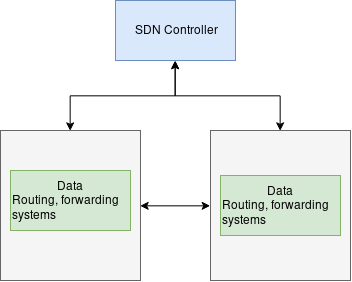
\includegraphics[width=.4\textwidth]{bib/network_sdn}\label{fig:net_sdn}}
      \caption {Traditional vs SDN network architecture}
    \end{figure}
\end{frame}

\begin{frame}
    \begin{figure}[!tbph]
        \centering
        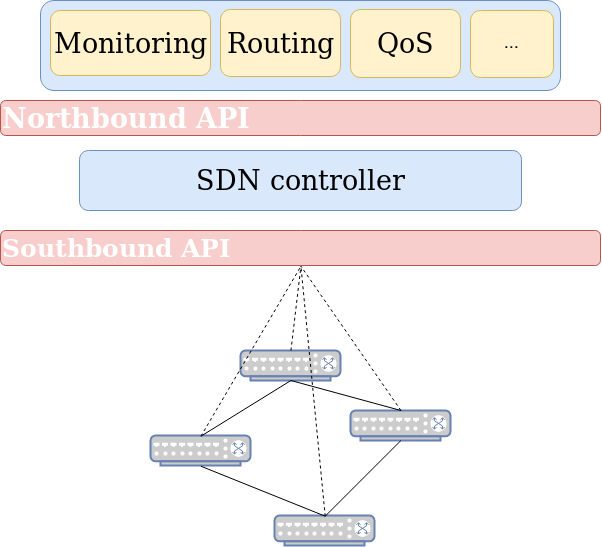
\includegraphics[width=.5\textwidth]{sdn/sdn_division}
    \end{figure}
    \begin{itemize}
        \item The SDN controller plays a central role in this architecture by connecting the network applications that connect to the Northbound interface to the
            networking devices running on the Southbound plane
    \end{itemize}
\end{frame}

%\begin{frame}{Basebox}
%\end{frame}

\begin{frame}{Basebox}
    \begin{figure}[!tbph]
        \centering
        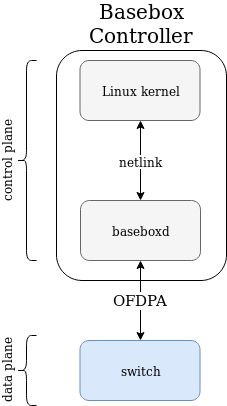
\includegraphics[width=.35\textwidth]{bisdn/baseboxd}
    \end{figure}

\end{frame}

\begin{frame}{Basebox}
    \begin{figure}[!tbph]
        \centering
        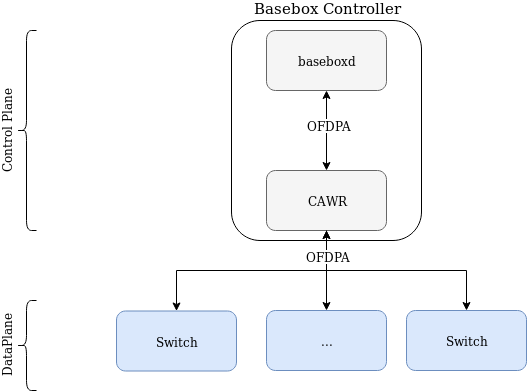
\includegraphics[width=.7\textwidth]{bisdn/cawr}
    \end{figure}
\end{frame}

\section{Problem}

\begin{frame}{Goals}
    \begin{itemize}
        \item Definition and implementation of a management stack for both controllers, to monitor port statistics and visualize topology changes
            \pause 
        \item Research and develop a solution for monitoring \textbf{elephant flows}
    \end{itemize}
\end{frame}

\begin{frame}{Elephant Flows}
    \begin{itemize}
        \item In typical Data Center Networks, their traffic characteristics show that \cite{mori_identifying_2004}:
            \pause
        \item For cloud data centers, the majority of traffic is internal to each rack
            \pause
        \item Link utilizations are low in aggregation and edge layers
            \pause
        \item Despite 90\% flows are small and last hundreds of milliseconds, total traffic volume is largely dominated by the remainder, called 
            \textbf{elephant flows} \cite{benson_network_2010}
    \end{itemize}
\end{frame}

\begin{frame}{Proposed Architecture}
        \begin{figure}
            \includegraphics[width=.7\textwidth]{proposed_work/proposed_system}
        \end{figure}
\end{frame}

\begin{frame}{Testing Environment}
    \begin{itemize}
        \item Due to the differences between the OF-DPA compliant hardware switches and the standard OpenFlow implementation used in the virtualised 
            network Mininet, testing the elephant flow detection mechanism proved impossible with Basebox, which led us to choosing a different controller
            \pause 
        \item The controller chosen was Floodlight, due to simplicity of installation and REST interface
        \item For development of the Graphical User Interface, the standard Basebox topology was used
    \end{itemize}
    \begin{figure}
        \includegraphics[width=.7\textwidth]{}
    \end{figure}
\end{frame}

\begin{frame}{Testing Environment}
    \begin{figure}
        \includegraphics[width=.7\textwidth]{meter_eleph/testing_setup}
    \end{figure}
\end{frame}

\section{Elephant Flow Monitoring}

\begin{frame}{Impact}
    \begin{figure}
        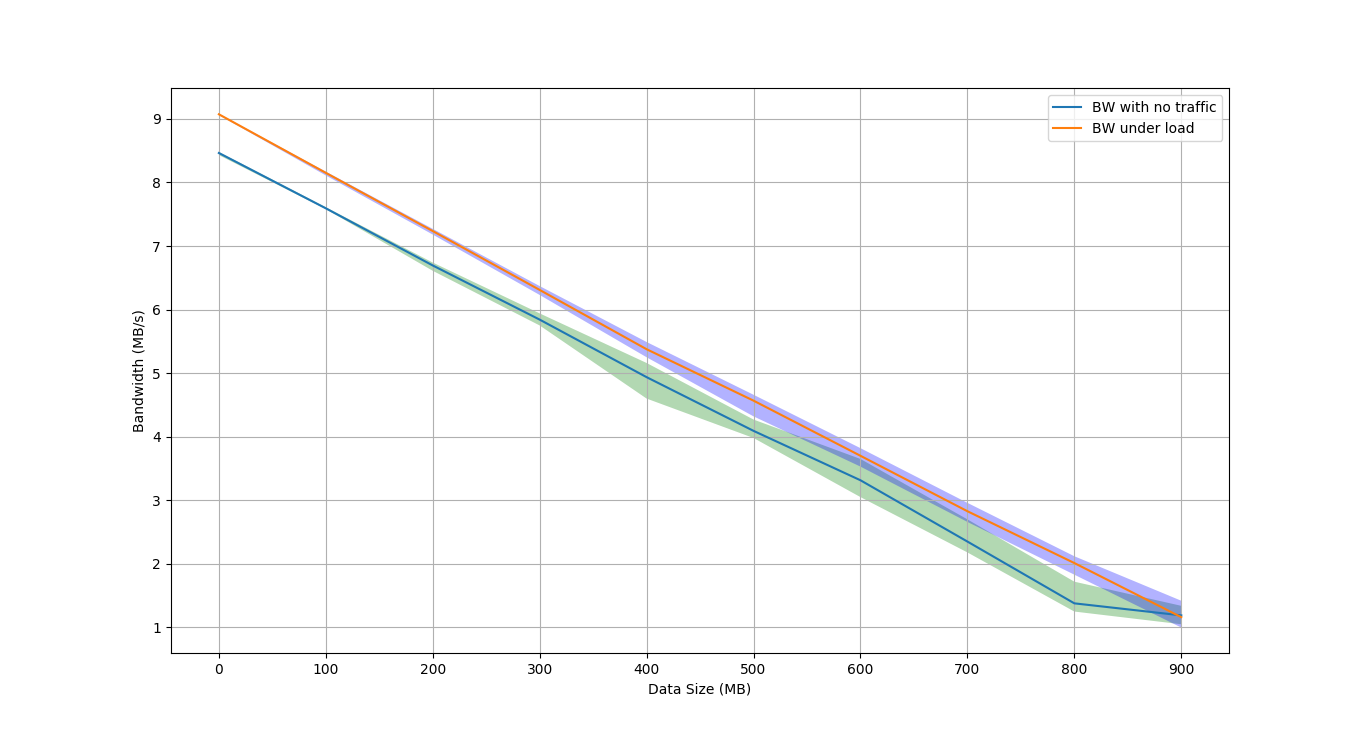
\includegraphics[width=1\textwidth]{meter_eleph/bandwidth_loss_per_data_size}
        \caption{The impact on the bandwidth of a link as the packet data sizes increase}
    \end{figure}
\end{frame}

\begin{frame}{Proposed Algorithm}
    \begin{algorithm}[H]
        \caption{Elephant Detection Algorithm - High Level} \label{alg:high_level}
        \begin{algorithmic}[1]
            \Procedure {Elephant Flow Detection}{}
                \State Initialization
                \Loop
                    \State Query controller
                    \State Error calculation
                    \State Prediction
                    \State Detection
                    \If {Detection}
                        \State Raise Alarm
                    \EndIf
                    \State wait 2 seconds
                \EndLoop
            \EndProcedure 
           \end{algorithmic}
    \end{algorithm}
\end{frame}

\begin{frame}{Initialization}
    \begin{figure}
        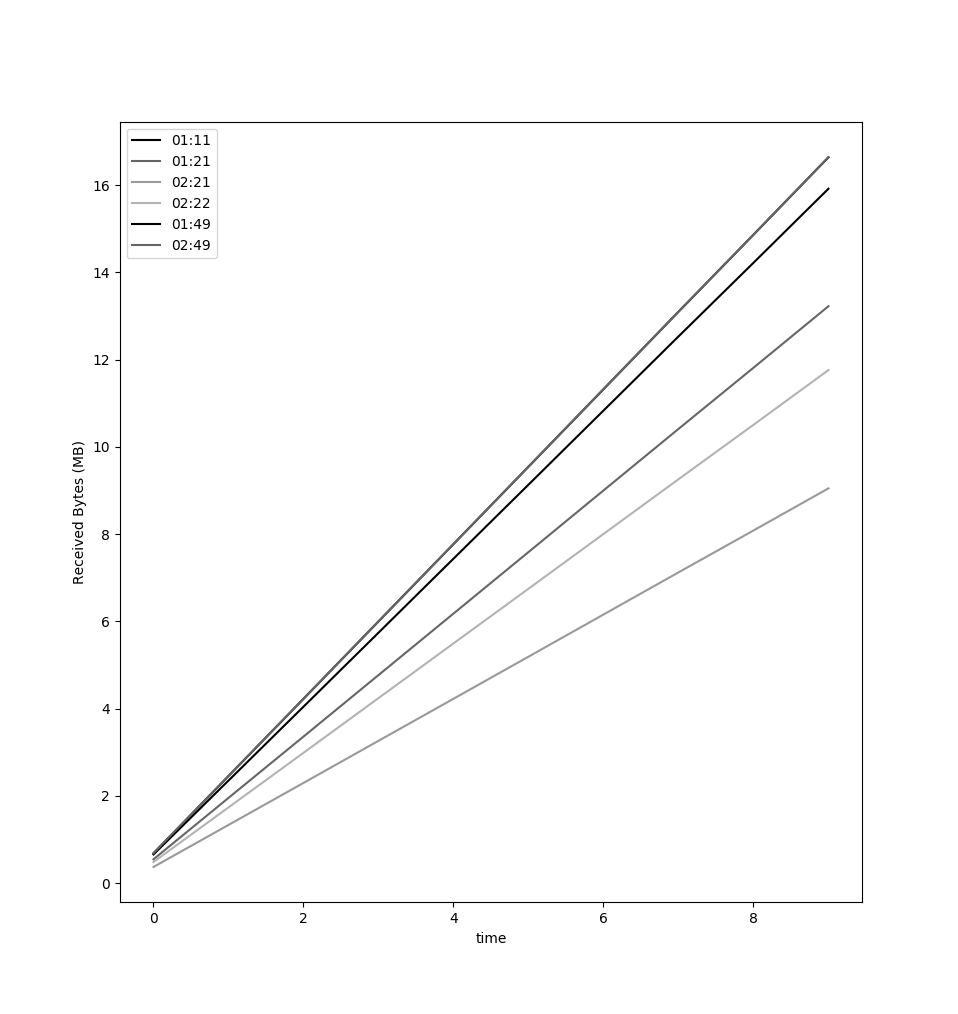
\includegraphics[width=.5\textwidth]{meter_eleph/init_period_lin}
        \caption{Initialization period plotted}
    \end{figure}
\end{frame}

\begin{frame}{Error calculation}
    \begin{figure}
        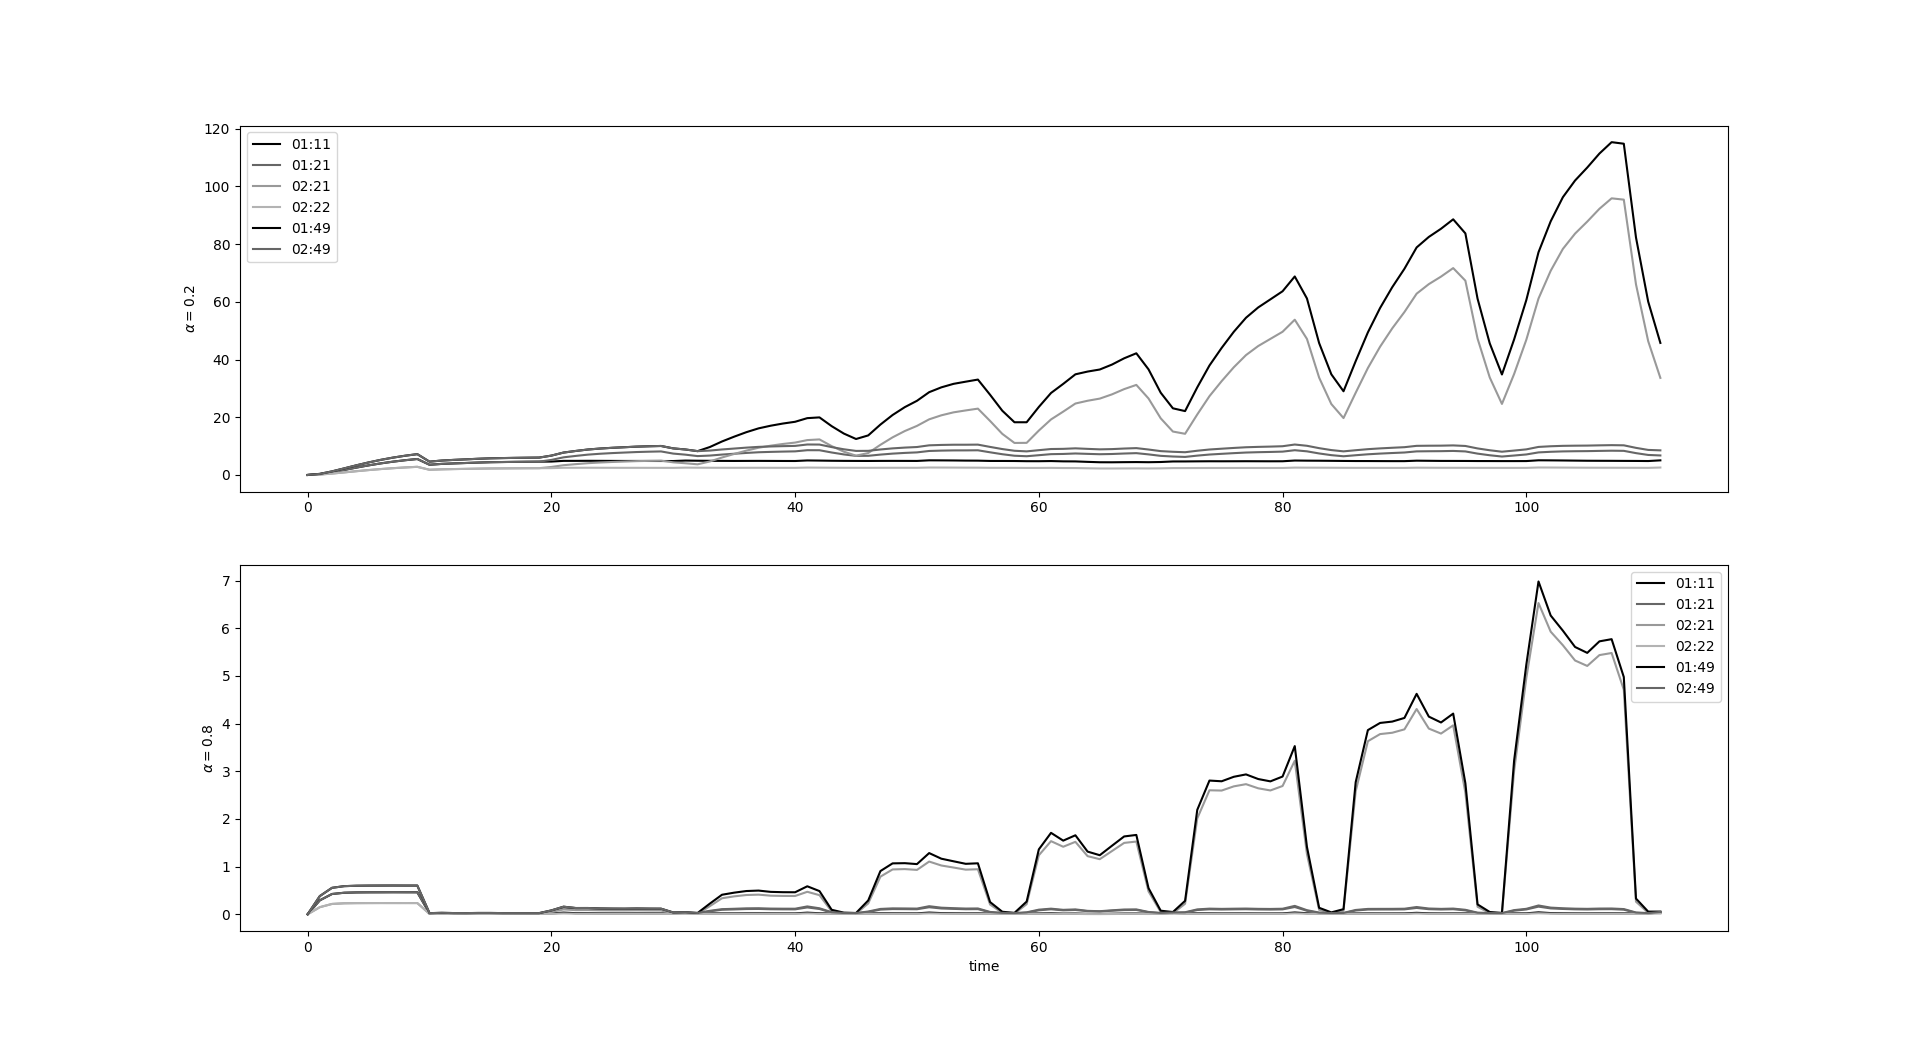
\includegraphics[width=1\textwidth]{meter_eleph/error_plot_sse}
        \caption{The prediction error obtained during the run time of the algorithm}
    \end{figure}
\end{frame}

\begin{frame}{Detection}
    \begin{figure}
        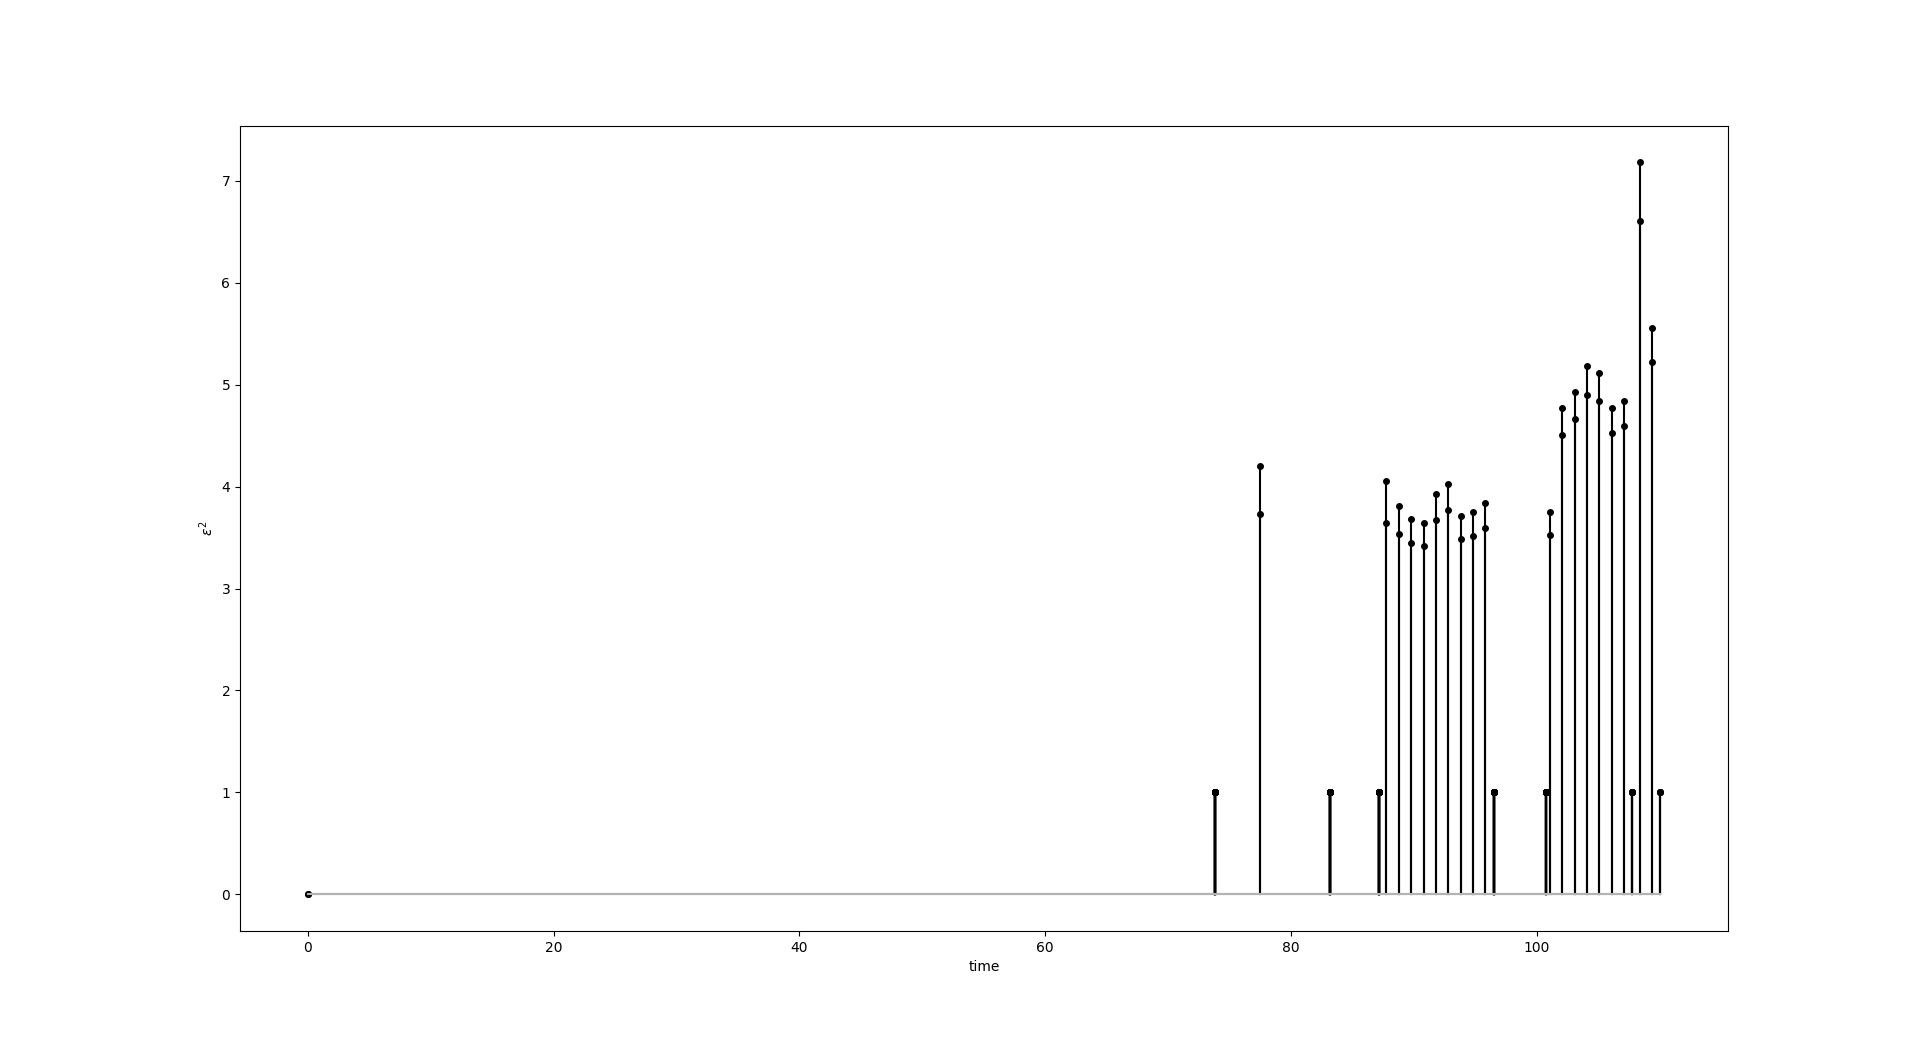
\includegraphics[width=1\textwidth]{meter_eleph/detect_dumb}
        \caption{First detection results}
    \end{figure}
\end{frame}

\begin{frame}{Detection}
    \begin{itemize}
        \item Previous detection results are not ideal, purely comparing the output
            of a value to a pre selected threshold, and raising several alarms
            even no change has been detected
            \pause
        \item The CUSUM algorithm is commonly used for change detection mechanisms employed
            in economics, health care, industrial engineering, ...
        \item Allows for keeping track of a parameter of an output of a process, and 
            compare it to pre selected thresholds, guaranteeing that the process is "in control"
    \end{itemize}
    \pause
    \begin{figure}
        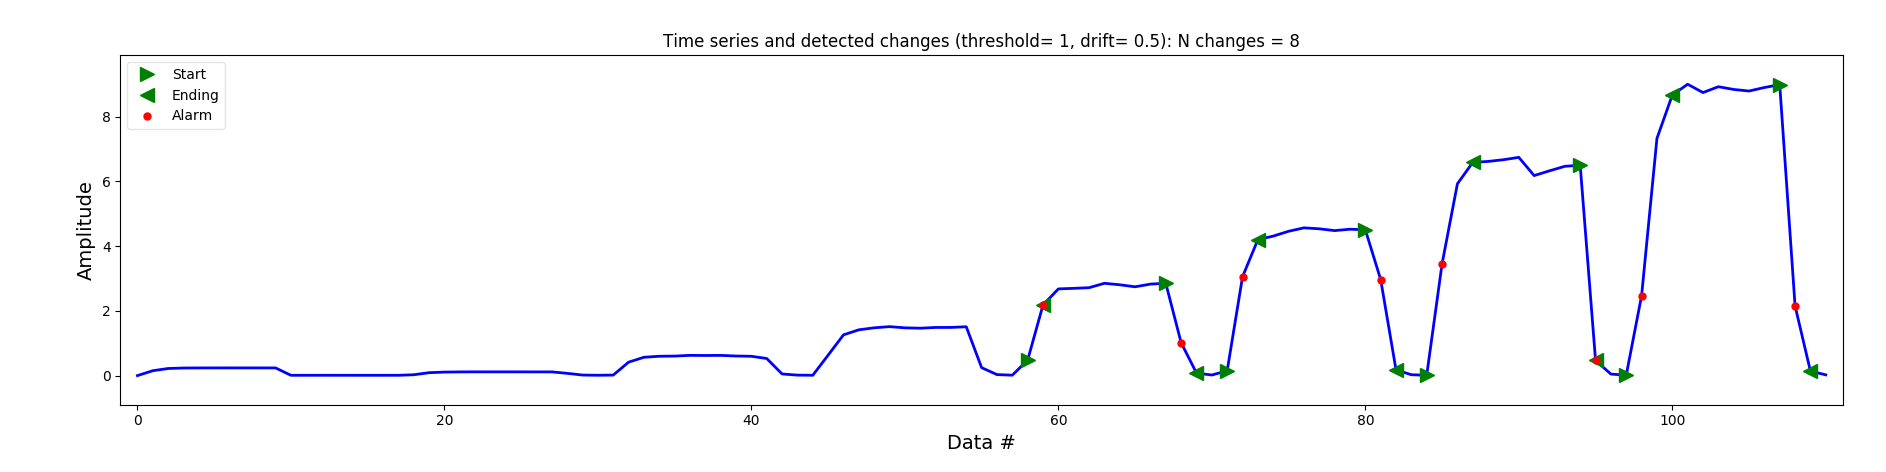
\includegraphics[width=1\textwidth]{meter_eleph/offline_cusum_output}
        \caption{Offline CUSUM output}
    \end{figure}
\end{frame}

\begin{frame}{Detection}
    \begin{itemize}
        \item Adaptation of the CUSUM algorithm to an online context is based on a sliding window
            method 
    \end{itemize}
    \pause
    \begin{figure}
        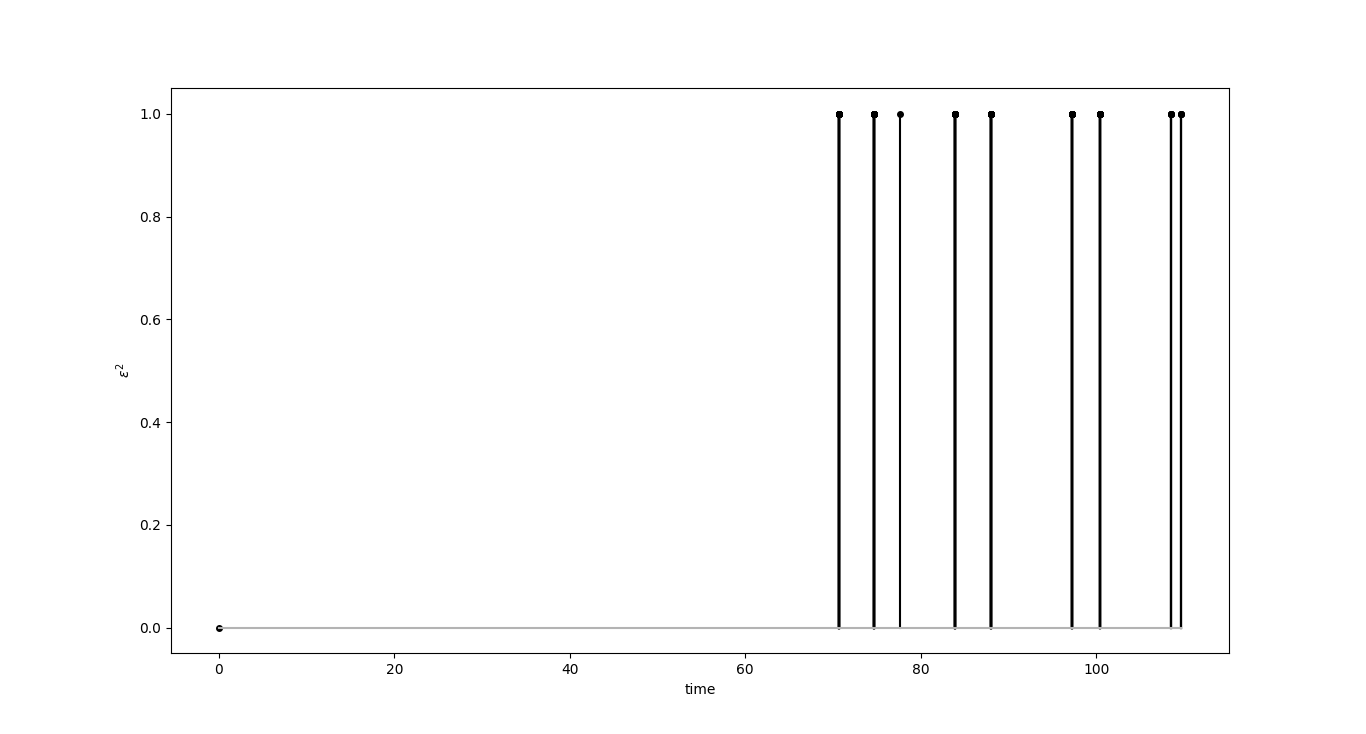
\includegraphics[width=.7\textwidth]{meter_eleph/online_cusum_output}
        \caption{Online CUSUM output}
    \end{figure}
\end{frame}

\begin{frame}{Evaluation of detection algorithm}
    \begin{figure}
        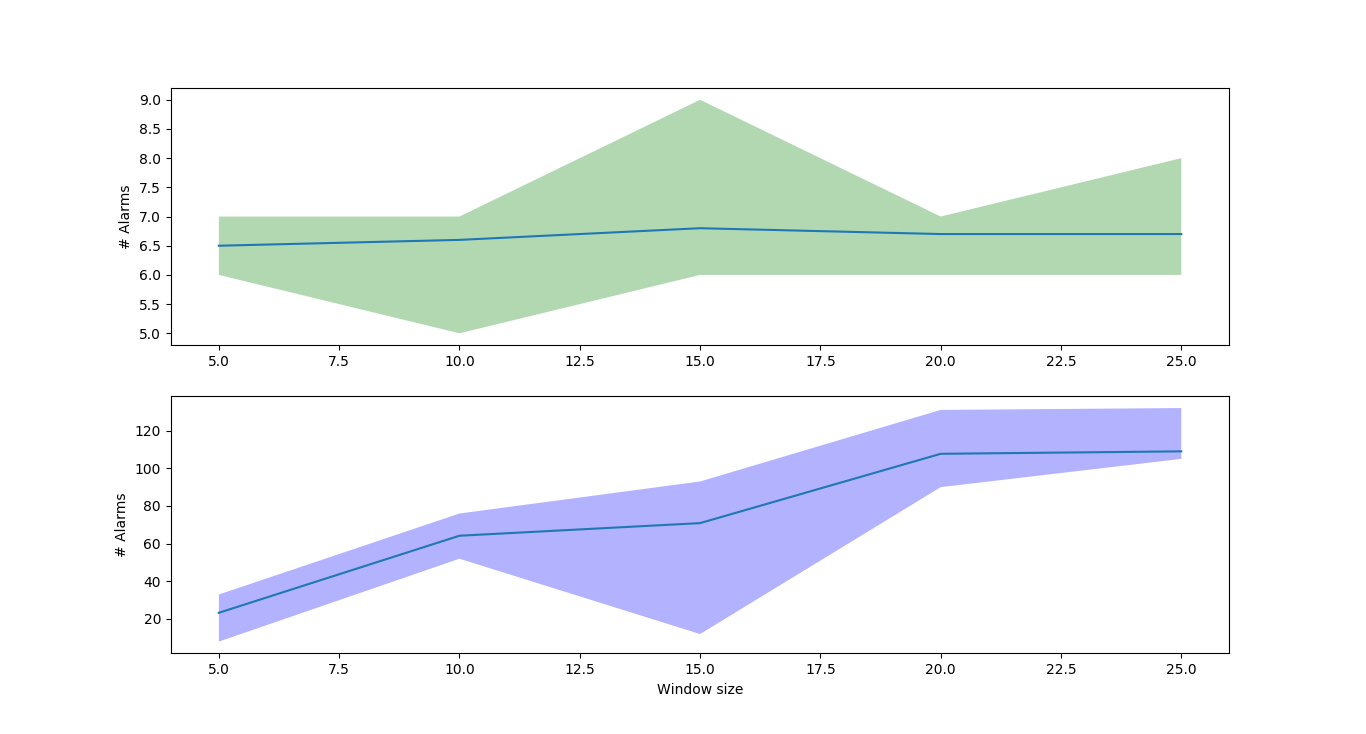
\includegraphics[width=.9\textwidth]{meter_eleph/evaluation_error}
        \caption{Number of alarms, optimized and non optimized}
    \end{figure}
\end{frame}

\section{Management API}

\begin{frame}{Design}
    \begin{itemize}
        \item By modifying the controllers to expose already available information like port statistics
            and link status, we created a simple GUI for simple visualization of this information
            \pause
        \item Based on a Remote Process Call framework, gRPC, we leverage this protocol's serialization model
            and RPC definition to create the endpoints between the GUI client and the controllers
            \pause
        \item We model the data according to standardized Yang data models, as defined by OpenConfig and IETF
            \pause
        \item The GUI client is a web page based on the Django Framework
    \end{itemize}
\end{frame}

\begin{frame}{Results}
    \begin{figure}[!tbph]
      \centering
      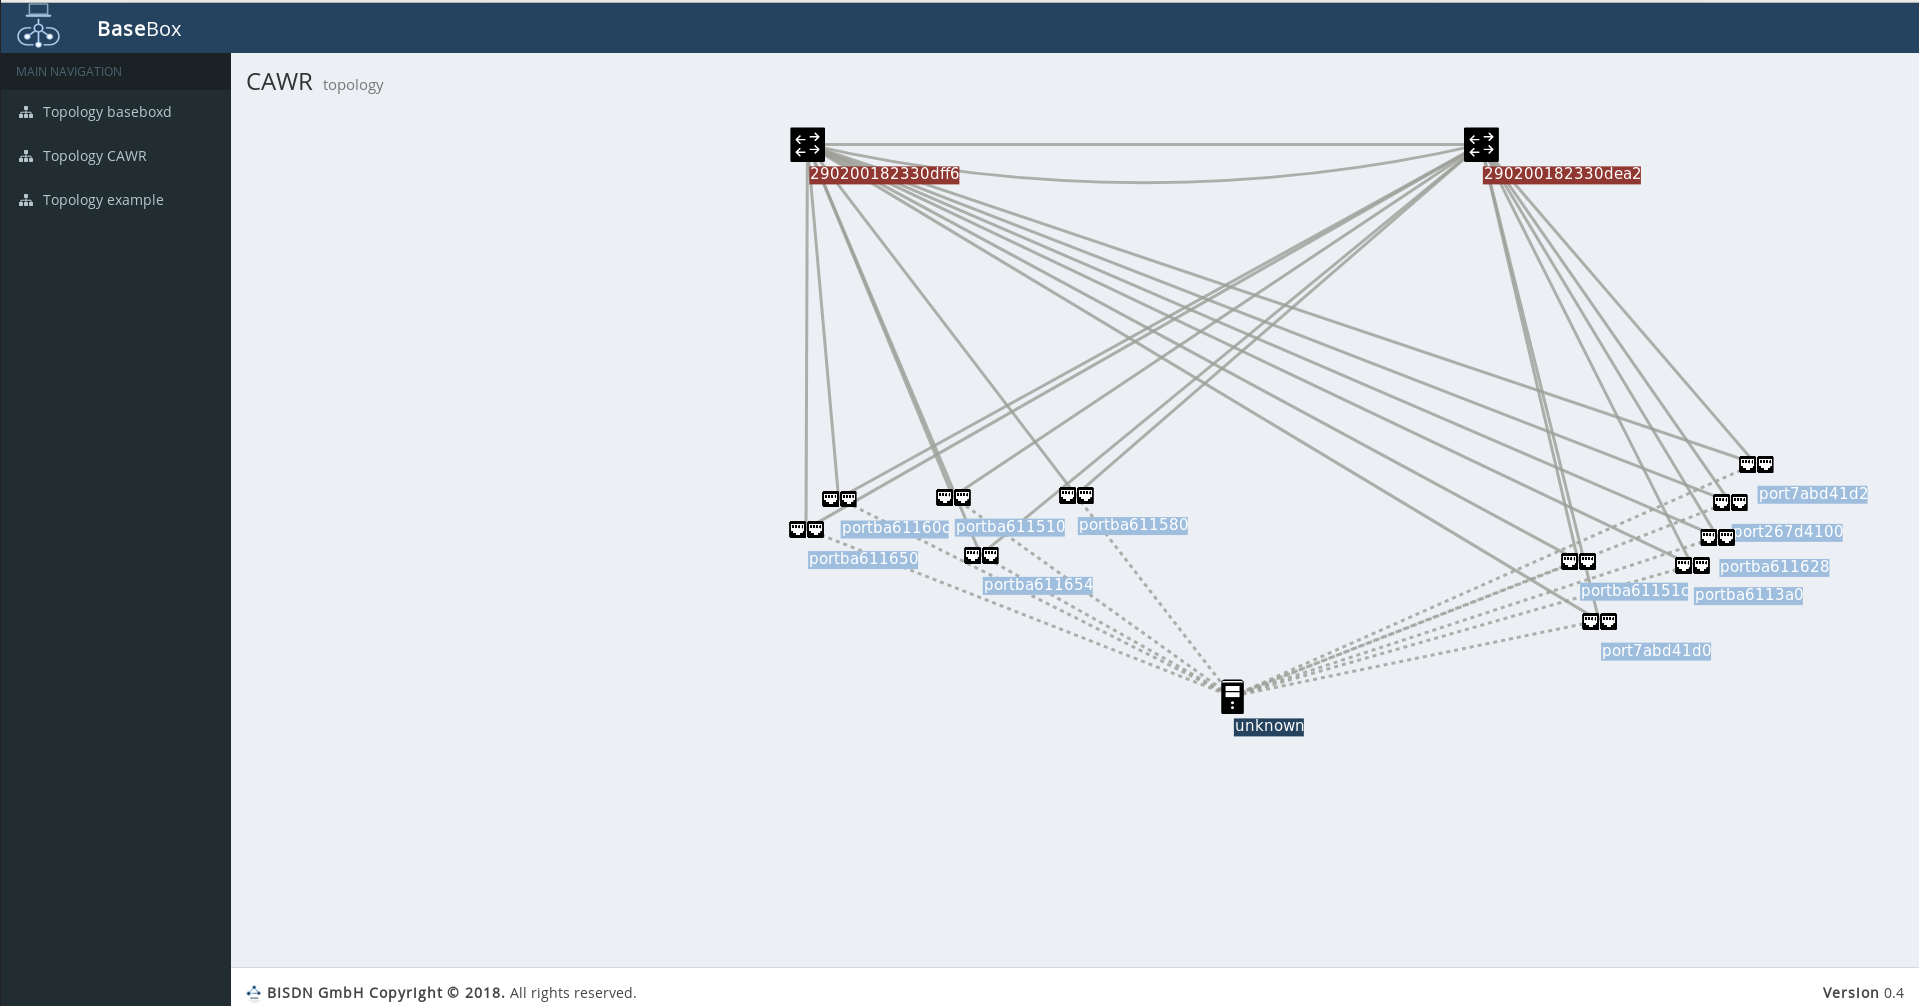
\includegraphics[width=0.8\textwidth]{bisdn/cawr_gui}
      \caption {CAWR topology, with the underlying switch topology}
    \end{figure}
\end{frame}

\begin{frame}{Results}
    \begin{figure}[!tbph]
      \centering
      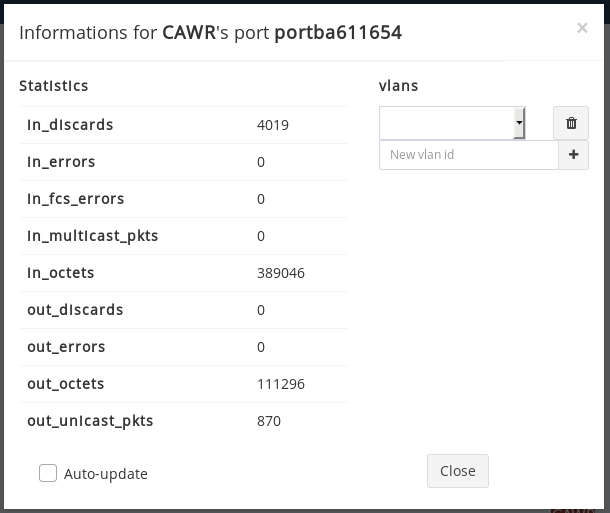
\includegraphics[width=0.7\textwidth]{bisdn/basebox_gui}
      \caption {baseboxd's statistics, with the statistics of a single port}
    \end{figure}
\end{frame}
\section{Conclusion}

\begin{frame}{}
    TBD
\end{frame}

\printbibliography
\end{document} 
%\begin{frame}{}
%\end{frame}
